\documentclass[titlepage]{article}
\usepackage[T1]{fontenc}
\usepackage[utf8]{inputenc}
\usepackage{color}
\usepackage{hyperref}
\usepackage{float}
\usepackage{datetime}
\usepackage{graphicx}
\usepackage{attachfile}
\usepackage[margin=3cm]{geometry}
\graphicspath{{./assets}}
\hypersetup{
	colorlinks=true,
	linktoc=all,
	linkcolor=black,
}

\title{Typeracer Project Specification \\ \large Software Engineering 1}
\author{Muratcan Akçay, Kamil Monicz,\\ Maciej Piętka, Marcin Wojnarowski}
\date{\monthname, \the\year}
	
\newcommand{\secref}[1]{{(Section \hypersetup{linkcolor=blue}\ref{#1})}}

\newcommand{\figref}[1]{{(Fig. \hypersetup{linkcolor=blue}\ref{#1})}}

\begin{document}

\maketitle

\tableofcontents
\newpage

\section{Introduction}

\subsection{Preface}

It is without question that typing is a crucial skill in the age of computers. We type to message our loved ones, to write a professional email, to calculate, or even to write specifications such as this one. While other solutions such as Speech-To-Text are gaining popularity, they will never be able to replace typing. Typing serves as the primary mean of communication with our computers.

Often times the skill of typing is implicitly assumed by employers; nowadays nearly all jobs require some sort of interaction with a computer. Lack of this skill can greatly hinder our performance on a day to day basis.

Typing ranges from being a required chore to be able to communicate thoughts with a computer to a fun, competitive activity.

\subsection{Existing work}

Typing game is not an new idea, in fact the term {\it Typing game} is a popular video game genre. During the age of internet many new typing games have emerged. Below we present the current most popular choice for typing games and its drawbacks.

A homonymous site by the name of \url{typeracer.com} is by far the most popular choice for competitive and casual typing. Similarly to our project, {\it typeracer.com} focuses on real-time multiplayer. However, it comes with some important drawbacks:

\begin{itemize}
	\item Proprietary -- Source is not available, cannot be tinkered with

	\item Commercial model -- Some feature are locked behind a paywall

	\item Single client -- server-client communication is not standardized, forced to use the provided client

	\item Single server -- there is only one true server, games over the local network cannot be hosted
\end{itemize}

These limitations are the primary areas which will be directly tackled in this project.

\subsection{Overview}

The goal of the Typeracer project is to create a multiplayer interactive typing game. The aim is to create a standardized game server which will be able to host games for any compliant client regardless of its technological stack. The following three rules are to be enforced by the project:

\begin{enumerate}
	\item Clients are interchangeable and can coexist -- a server can host a game for any compliant client as well as different clients can be in the same game.

	\item Hostability -- server can be easily self hosted, whether that would be on a private server or on a local network.

	\item Real-time -- multiplayer games are updated in real time
\end{enumerate}

The game itself simply serves as a trainer and entertainer (if one enjoys fast typing). The game consists of a single input field, a text with the paragraph to be typed and the progress of all players \figref{fig:overview}.

\begin{figure}[ht]
	\centering
	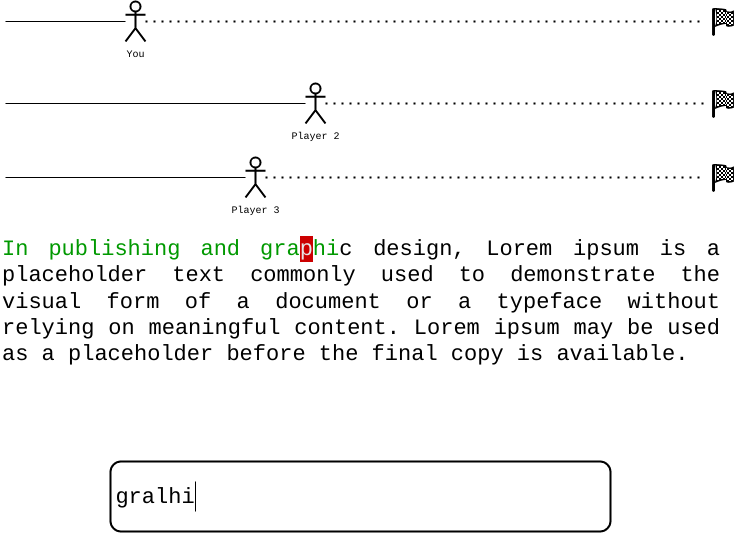
\includegraphics[width=0.79\textwidth]{overview.png}
	\caption{Overview of the game}
	\label{fig:overview}
\end{figure}

However before one can reach the game, the preferred game server has to be picked. Afterwards player waits in a lobby where other players can join the room. To help pass time, the lobby has an integrated chat.

Everything is managed by a running server and games can be moderated by admins. Best scores are kept in a leaderboard which it too can be moderated by an admin.

To sum up, this project consists of three components:

\begin{enumerate}
	\item Client -- Interacts with players, plays games
	\item Server -- Hosts games
	\item Admin panel -- Interacts with admins, manages games
\end{enumerate}

\subsection{Nomenclature} \label{nomenclature}

The following terms will be used throughout the specification, some come from the typing world and some from the technical one.

\begin{itemize}
	\item {\bf WPM} -- Words Per Minute, primary typing metric. Defines the average amount of correctly typed words per minute.

	\item {\bf Typer} -- Typeracer player.

	\item {\bf DNF} -- Did Not Finish, equivalent with disqualification.
\end{itemize}

\section{Requirements}

To start, a strict set of requirements has to be defined. The requirements are expressed in User Stories, a list of functional requirements, and finally other non-functional ones. Clearly defined requirements are crucial for a complete and cohesive system, which has to be the case in Typeracer due to its interchangeable nature.

\subsection{User Stories}

User Stories are written from the user's perspective (whether that would be a player or admin) and describe the expected results together with some acceptance criteria.

\subsubsection{Player user stories}

The most important actor is the player, after all all components are built with the player in mind. The following set of user stories will help illustrate what a user expects from the game.

\newcommand{\AC}{\subitem AC. }

\begin{enumerate}
	\item
	      As a player, I want to play a competitive typeracer game so that I can compare my typing skills against other people, increase my typing skills and have fun.
	      \AC
	      The game accepts multiple players together to type a block of text and race against each other and announces the order of completion.

	\item
	      As a player, I want to set my playerName so that other players can see my name on the leaderboard if I score a high score.
	      \AC
	      The game allows players to set their names and use them for displaying the leaderboard.

	\item
	      As a player, I want to see the daily and all-time high scores so that I can compare my skill level to the best players.
	      \AC
	      The game provides functionality to display the top ten daily/all-time scores in words per minute format.

	\item
	      As a player, I want to see how many players I'm playing against and the placement of all players during the game so that I can compare my skill position to the players I am playing with.
	      \AC
	      The game shows the player's position during the game.

	\item
	      As a player, I want to see the placement of all players at the end of the game so that I can compare my skill level to the players I played with.
	      \AC
	      The game shows each player's placement and score in words per minute format at the end of each game.

	\item
	      As a player, I want to choose which regional server I want to play on so that I will have the least latency during the game.
	      \AC
	      The game allows for choosing from three regional servers (NA, Europe, Asia) to play on at the beginning.

	\item
	      As a player, I want to chat with the other players after a game is over so that I can communicate with the other players and express my opinions.
	      \AC
	      The game displays a chat box at the end of each individual game where the players can chat until the next game begins.
\end{enumerate}

\subsubsection{Admin user stories}

The second actor is the admin which can moderate various aspects of the server and clients. The following list enumerates expectations of an admin with regards to their admin panel.

\begin{enumerate}
	\item
	      As an admin, I want to search the content database so that I can see which entries contain the search phrase I enter and remove that entry if I want.
	      \AC
	      The game allows admins to search the database and displays the entries containing the search phrase.

	\item
	      As an admin, I want to add or remove content to the game so that I have control over the texts that will be shown to the players.
	      \AC
	      The game allows admins to add or game content to the database by pasting in a text box or importing as a .txt file.

	\item
	      As an admin, I want to edit the displayed announcement text so that players are informed about important events such as server downtime or high score reset dates.
	      \AC
	      The game allows admins to modify the announcement text displayed on the main game window.

	\item
	      As an admin, I want to shut down the game service so that I can make changes in the configuration of the game without problems.
	      \AC
	      The game allows admins to shut down the game service.

	\item
	      As an admin, I want to restart the game service so that changes made can take effect and any existing errors can be remedied.
	      \AC
	      The game allows admins to restart the game service.

	\item
	      As an admin, I want to reset the leaderboard so that a new game season can be started with a blank all-time leaderboard allowing new players to compete for the high scores.
	      \AC
	      The game allows admins to reset the leaderboard.

	\item
	      As an admin, I want to adjust the queue duration so that I can manage how long players have to wait before a game starts.
	      \AC
	      The game allows admins to adjust the waiting queue duration.

	\item
	      As an admin, I want to adjust the DNF (did not finish) duration so that I can manage how long players have to wait before a game ends, even if one of the players never finishes typing the text.
	      \AC
	      The game allows admins to adjust the DNF duration.
\end{enumerate}

\subsection{Functional requirements}

To be more specific, a list of core functional requirements is listed below.

\begin{itemize}
	\item The players can set their player names before starting to play the game
	\item The players can see the daily and all-time leaderboards where high scores are displayed.
	\item While a game is being played, the players can see how many players are playing and their placement among other players in real-time.
	\item When a game ends the players can see their final placement among other players that participated in the game and their typing speed in wpm (words per minute).
	\item The players can choose which regional server they want to play on to mitigate the effects of latency.
	\item The admins can log in to the admin panel using an admin passphrase
	\item The admins can edit the announcement text which will be displayed to the players.
	\item The admins can shut down the game service
	\item The admins can restart the game service
	\item The admins can adjust the waiting queue duration that counts down before the start of each game
	\item The admins can adjust the did not finish duration that defines the max. Time a game will last
	\item The admins can view the content database to see the entries sorted by date added
	\item The admins can search the content database to find all entries containing a specific search phrase
	\item The admins can remove an entry from the database
	\item The admins can add an entry to the database by pasting the text in a text box or importing a .txt file
	\item The admins can reset the all-time leaderboards
\end{itemize}

\subsection{Non-Functional requirements}

Finally, a set of non-functional requirements has to be presented to further describe the vision.

\subsubsection{Usability}

\begin{itemize}
	\item The service is available in English, for all users with an Internet/LAN connection.
	\item The user interface for the players is minimalistic, allowing only keyboard input, clear and easy to use.
	\item The user interface for the admins is minimalistic, allowing both mouse and keyboard input, clear and easy to use.
\end{itemize}

\subsubsection{Reliability}

\begin{itemize}
	\item The service will have at max 5\% of downtime.
	\item The service will be logging any encountered errors.
	\item The service will be restored in maximum of 1 day after a fatal error.
\end{itemize}

\subsubsection{Performance}

\begin{itemize}
	\item The service will support at least 1000 concurrent players on each server.
	\item The service can be scaled to support more users at a time.
\end{itemize}

\subsubsection{Supportability}

\begin{itemize}
	\item Both the player and admin components of the system will only be web-based and run on latest versions of Chrome, Firefox and Microsoft Edge browsers.
\end{itemize}

\newpage

\subsection{Use case diagram}

To sum up the requirements in a visual form, which will give a rough idea of how the usage should flow.

\begin{figure}[ht]
	\centering
	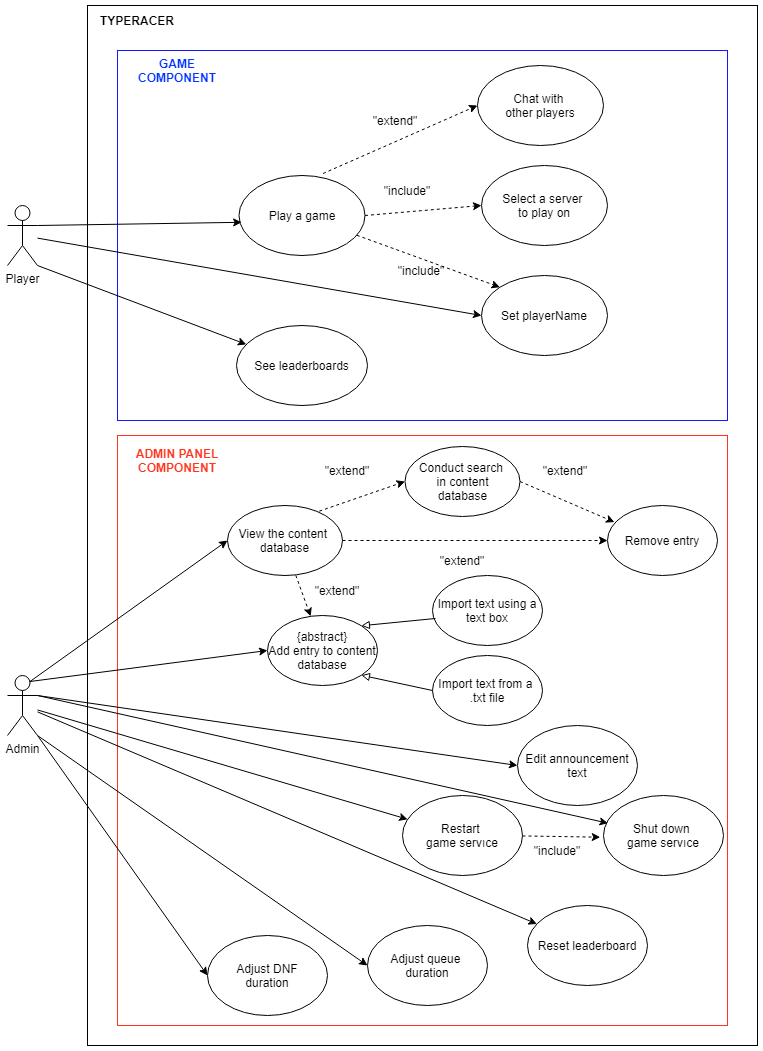
\includegraphics[width=0.75\textwidth]{use_case_diagram.png}
	\caption{Typeracer use case diagram}
	\label{fig:usecase-diag}
\end{figure}

\newpage

\section{Design}

In this section system's behavior and expected states are described.

\subsection{Class diagram}

The system can be split into few core components \figref{fig:class-diag}:

\begin{itemize}
	\item {\bf Player} -- It has to be able to select a server to which it will be able to later join a game. A player can also set its name as well as show the leaderboard.
	\item {\bf Chat} -- The chat module boils down to being able to send and receive messages.
	\item {\bf GameService} -- Manages starting and ending games. Additionally it can accept incoming connections and drop when needed. Whenever needed, it can also update the leaderboards.
	\item {\bf Lobby} -- Once players are in the lobby they are managed by the lobby class where the queue can be started. It can also control which component is being shown: announcement, chat, and leaderboard.
	\item {\bf Announcement} -- Can only be retrieved, or changed by the admin.
	\item {\bf Admin} -- Controls other services. It can start, stop, or restart the server. It can authenticate the admin by letting them login but also log out. Admin can also alter the dnf countdown, the queue countdown as well as change the announcement text. It can also inspect the leaderboard.
	\item {\bf Leaderboard} -- A leaderboard can either be daily or all time. Both of them can be modified: resetting to a clean slate, adding a record to a leaderboard and getting the leaderboard.
	\item {\bf ContentManager} -- Allows adding and deleting texts that will be typed by the players. Texts can be added either as a raw string or from a text file which will include many texts separated by some delimiter. Finally, it allows for picking a random text.
\end{itemize}

\begin{figure}[H]
	\centering
	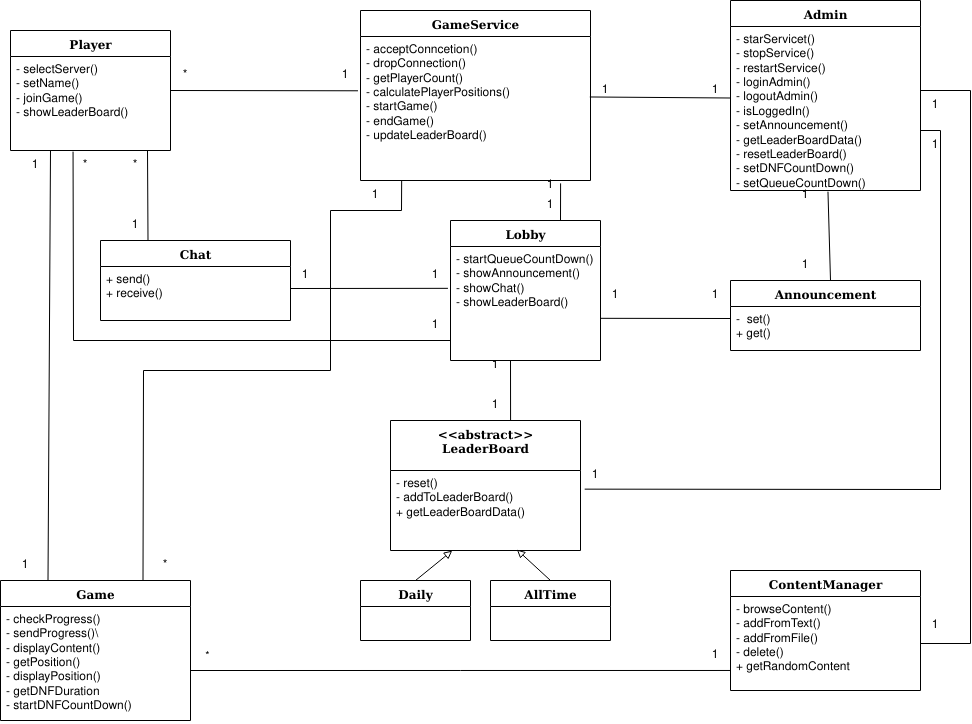
\includegraphics[width=0.79\textwidth]{class_diagram.png}
	\caption{Typeracer class diagram}
	\label{fig:class-diag}
\end{figure}

\subsection{State diagrams}

States of Typeracer are well defined, we can expect a fixed set of states.

\subsubsection{Server}

Server has a small amount of states \figref{fig:state-server}. Its responsibility is to accept incoming requests and handle them. Before receiving a request the server is in a waiting state. Once a request arrives it has to handle it, no matter whether the handling is successful or not, a response has to be sent back. In case of an error, it should be logged.

\begin{figure}[H]
	\centering
	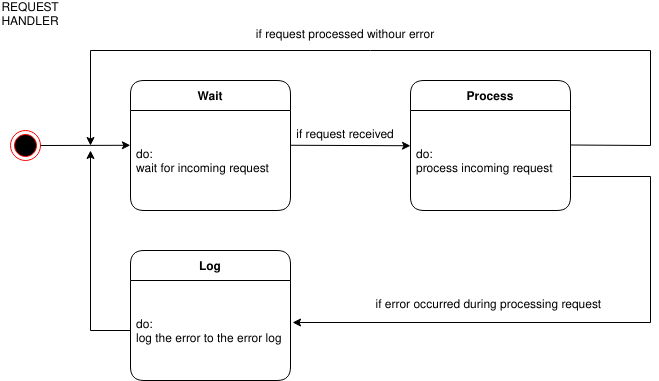
\includegraphics[width=0.79\textwidth]{state_diagram_server.png}
	\caption{Server's state diagram}
	\label{fig:state-server}
\end{figure}

\subsubsection{Admin panel}

Admin's state \figref{fig:state-admin} is the most complex due to the fact that many components can be altered resulting in many different states. The admin panel is guarded by a login screen which requires admin privileges. Once authorized, admin can browse many sub-pages in which they can change the behavior and look of the game. At any time, pressing the logout button brings the admin back to the login screen

\begin{figure}[H]
	\centering
	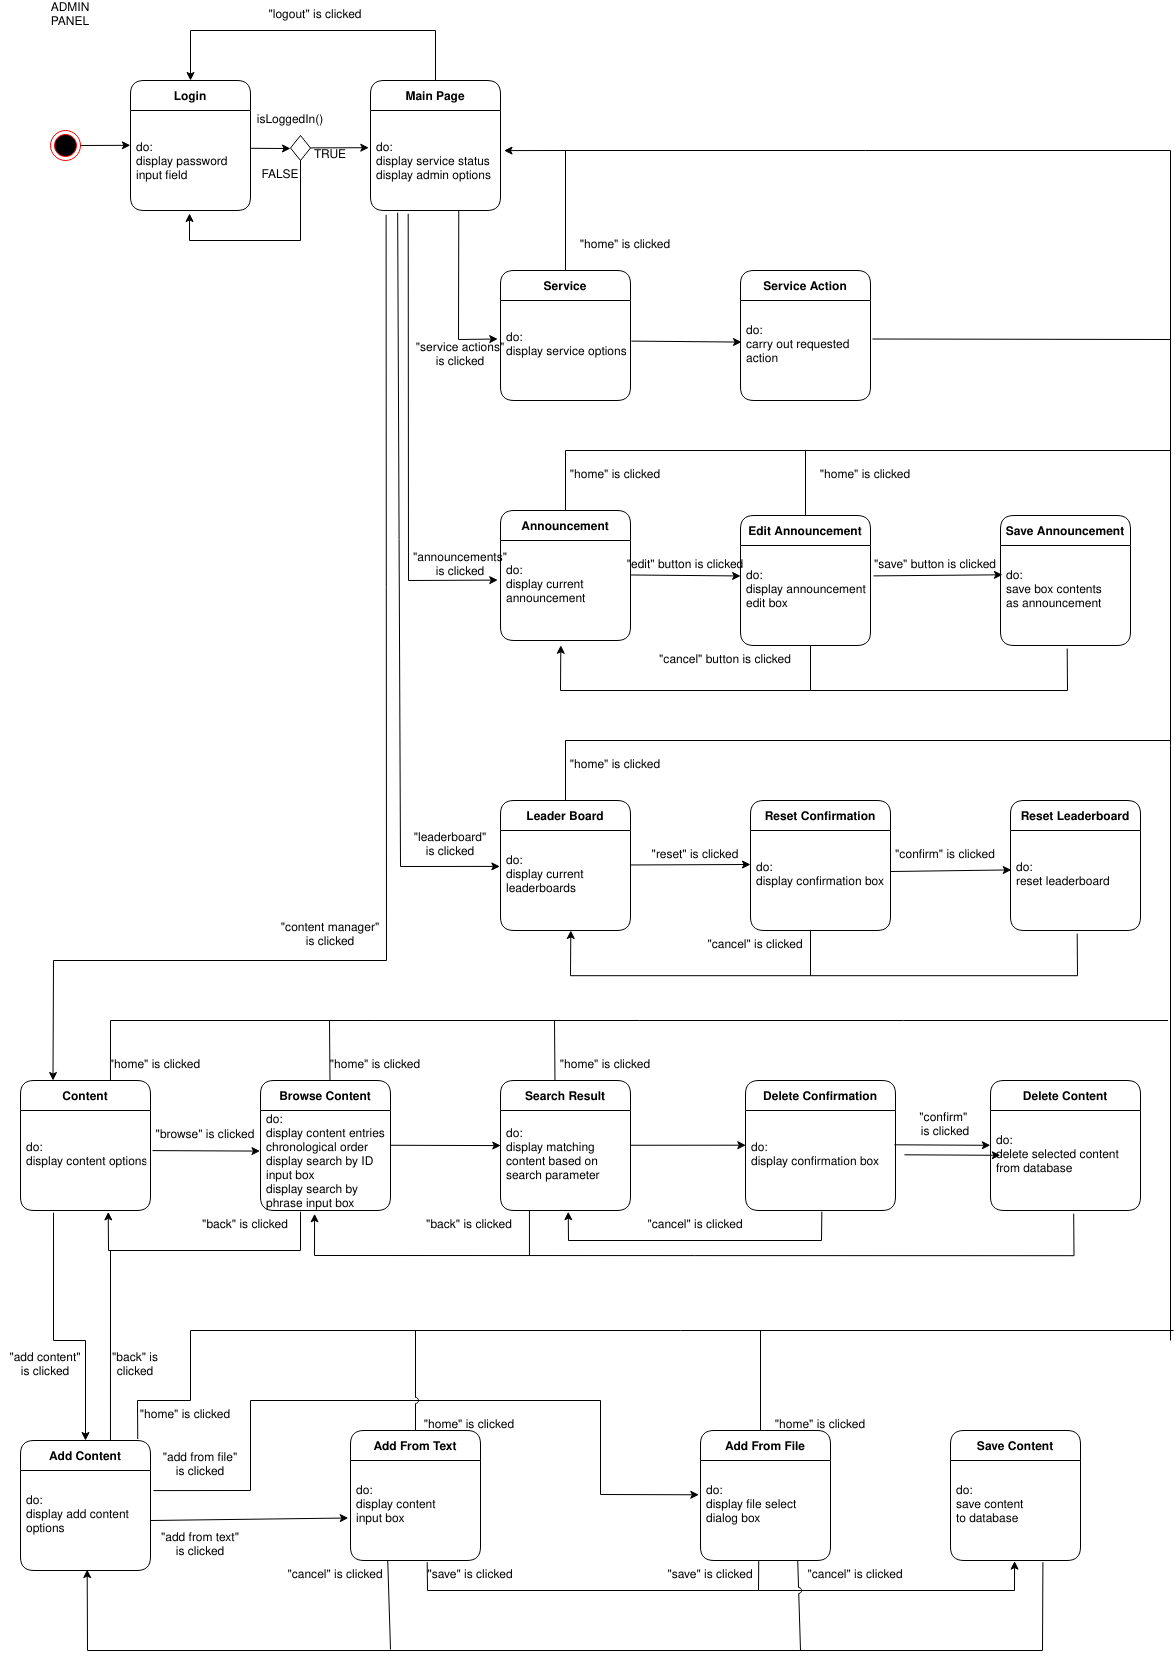
\includegraphics[width=0.79\textwidth]{state_diagram_admin.png}
	\caption{Admin's state diagram}
	\label{fig:state-admin}
\end{figure}

\subsubsection{Client}

Client's state is responsible for tracking player's progress and the usage flow. Three separate entities can be identified: Player, Lobby, and Game.

The player state \figref{fig:state-client-player} focuses on the states happening at the very beginning when the client is started. At first the user is prompted to enter their username, once it is confirmed and validated to be correct the user is redirected to a place where a game server can be chosen. Otherwise, the user stays in the set username screen until it is valid.

When selecting a server the only error state is a connection error. If it occurs the user is allowed to pick a game server again until success. Once a connection is successful user is moved to the lobby.

\begin{figure}[H]
	\centering
	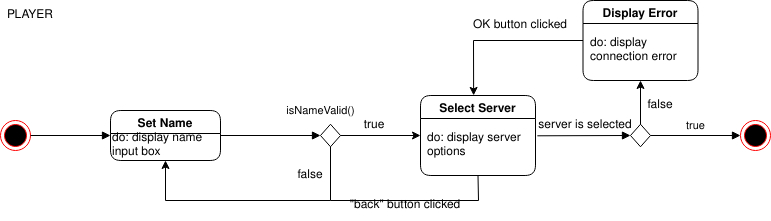
\includegraphics[width=0.79\textwidth]{state_diagram_player.png}
	\caption{Client's player state diagram}
	\label{fig:state-client-player}
\end{figure}

In the lobby \figref{fig:state-client-lobby} a countdown is ran in the background. Once it reaches zero, we exit the lobby and move to the game. Before that, there are two concurrent states: Lobby and Chat/Leaderboard. In the lobby the queue is displayed together with a announcement controlled by the admin. Chat and leaderboards are interchangeable and cannot be present at the same time. Leaderboards are spit into daily and all-time.

\begin{figure}[H]
	\centering
	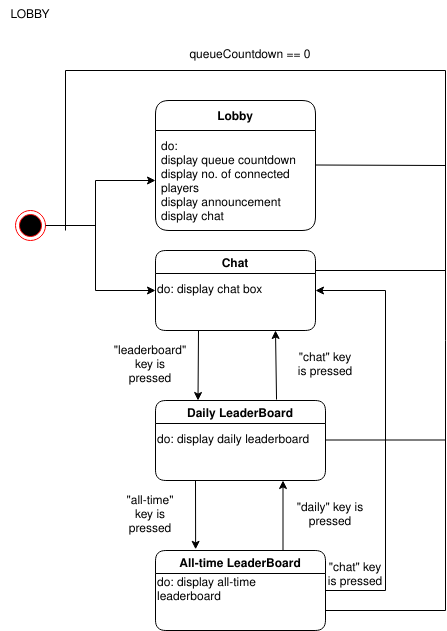
\includegraphics[width=0.79\textwidth]{state_diagram_lobby.png}
	\caption{Client's lobby state diagram}
	\label{fig:state-client-lobby}
\end{figure}

Finally, in the game section \figref{fig:state-client-game}, as the name suggests, the game takes place. Here the state is rather constant and is changed only if the game countdown reaches zero (which results in a DNF) or when every player finishes typing the text. During the game, the progress of other players is displayed, and the user advances through their text by typing consecutive words.

\begin{figure}[H]
	\centering
	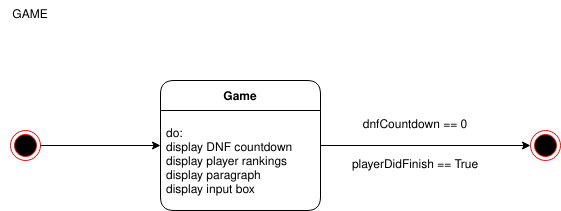
\includegraphics[width=0.79\textwidth]{state_diagram_game.png}
	\caption{Client's game state diagram}
	\label{fig:state-client-game}
\end{figure}

\subsection{Activity diagrams}

In this section the main user activity of playing a game is described. This activity consists of connecting to the server, waiting for a game to start, playing a game, viewing the leaderboard and either choosing to play another round or disconnecting from the server.


\begin{figure}[H]
	\centering
	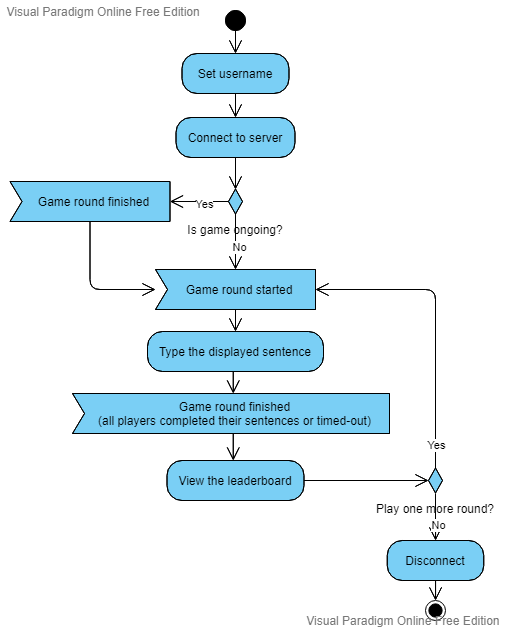
\includegraphics[width=0.79\textwidth]{activity_diagram_game.png}
	\caption{Game's activity diagram}
	\label{fig:game-activity}
\end{figure}


The action starts with the user being prompted to enter a username of their choosing \figref{fig:game-activity}. After a name is entered, the user is redirected to a game server selection screen where they can choose which game server they want to join in order to play a game.

Once a server is selected by the user and the connection to the server is established, the user is redirected to a lobby screen. If a game is in progress the user waits in this lobby screen until the countdown reaches zero and the ongoing game is finished. After the game is finished a new game is started and the user is shown a sentence which they must type. The game ends for the user when they finish typing the displayed text without any errors or when the game countdown reaches zero. At the end of the game a leaderboard is displayed with the best scores and the user may select to play another round or quit.

\begin{figure}[H]
	\centering
	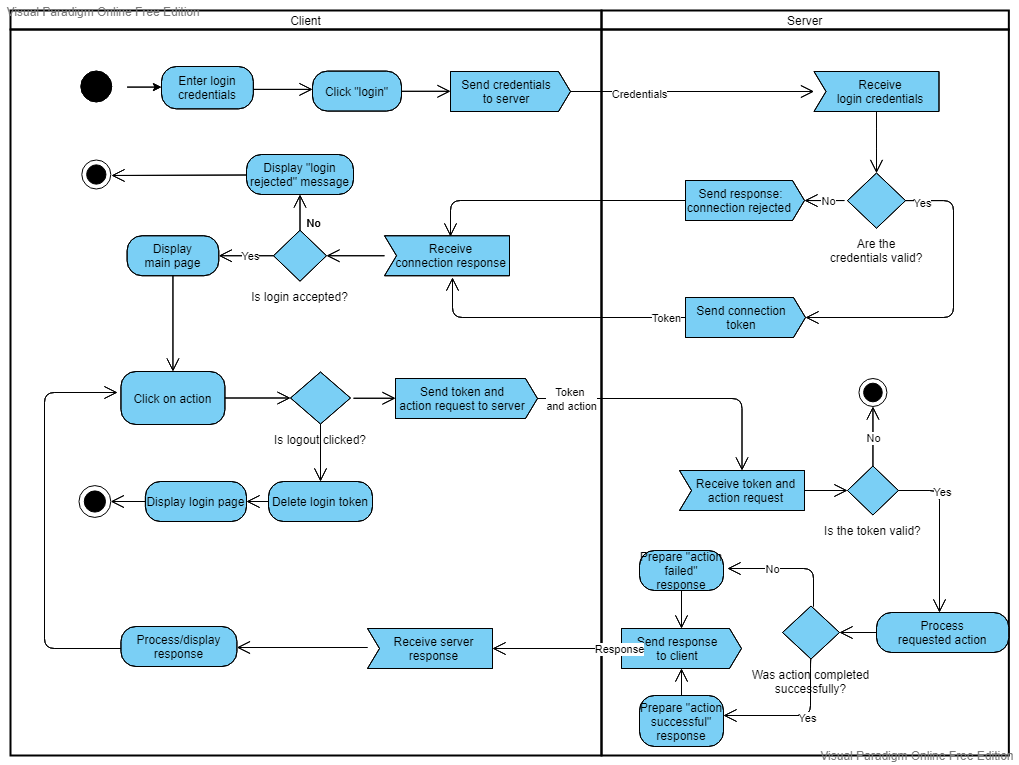
\includegraphics[width=0.79\textwidth]{activity_diagram_admin.png}
	\caption{Admin's activity diagram}
	\label{fig:admin-activity}
\end{figure}


When a user connects to the admin panel the login screen is displayed, asking for the login credentials \figref{fig:admin-activity}. Only authorized admins are allowed to log in to the admin panel since this component can be used to alter the functionality of the game by changing the database of the stored texts, countdown durations, etc. When the user enters the credentials these are sent to the server. The server receives the credentials and confirms that they are valid. If the credentials are not valid the user is informed about this situation and notified through a "login not accepted" message. If the credentials are valid then the server sends a login token to the client, to be used in all further communications in order to confirm that actions are taken by an authorized admin. Then the user is taken to the main page of the admin console where they can choose to perform any of the actions provided for the admins. These actions are detailed in the state diagrams. Once the user selects an action they want to carry out, a request, along with the login token is sent to the server. The server confirms that the token is valid before processing the requested action. The outcome of the action, whether it's successful or failed, is also notified to the user. The user can perform multiple actions until they log out. When a user clicks logout the token is deleted from the client side.


When a player types in the chat \figref{fig:chat-activity} and presses the return key a signal is sent to the server via the established websocket connection, containing the message and the player's name. The Server then proceeds to validate the message, making sure that it does not contain any blacklisted words or phrases. If the message is not valid then it is replaced with a \texttt{"<message deleted>"} text, otherwise it is copied as it is to create a new text. This new text is then copied to the list of all messages and is multicast to all clients at once. A client receiving a new message from the server displays it at the bottom of the chat windows as a new message, along with the name of the player that sent it.

\begin{figure}[H]
	\centering
	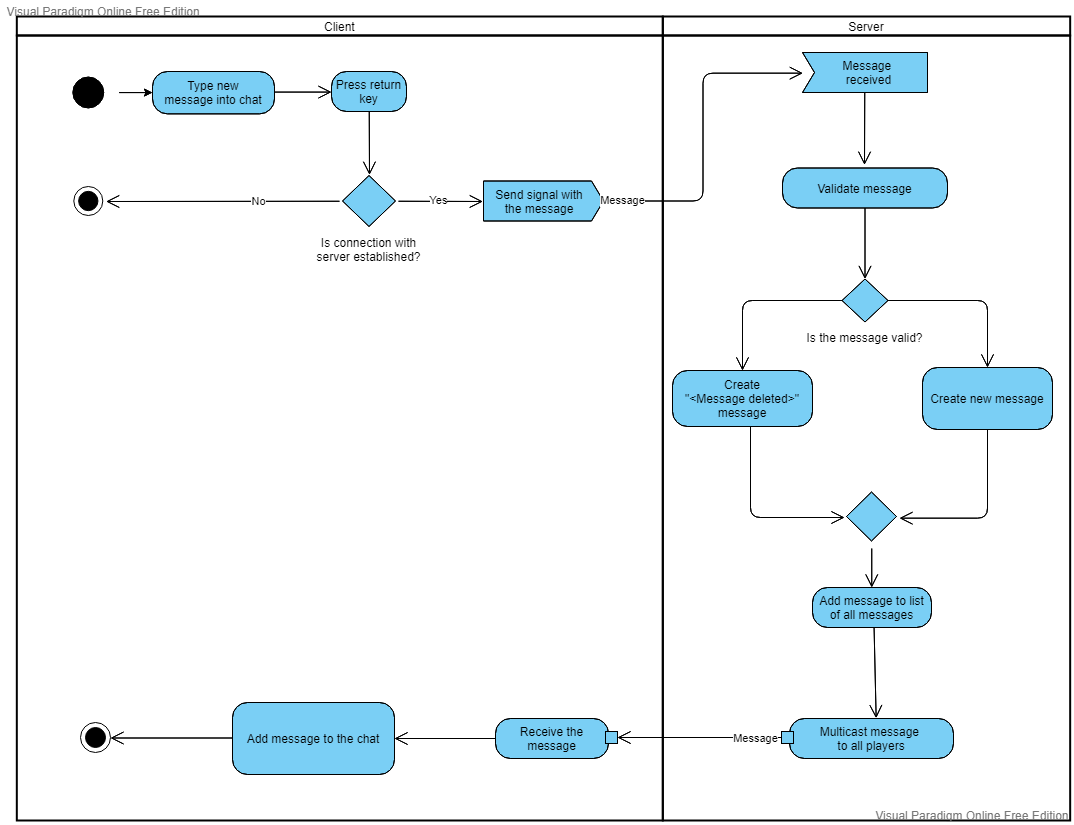
\includegraphics[width=0.79\textwidth]{activity_diagram_chat.png}
	\caption{Chat's activity diagram}
	\label{fig:chat-activity}
\end{figure}

When a player types in the input box, the client app checks to see if a word was typed with no mistakes \figref{fig:progress-activity}. If this is the case a signal is sent to the server via the established websocket connection, containing the progress of the player. The Server then proceeds to process this information and based on the time elapsed and the number of words typed correctly in the input box, re-orders the progress states of all connected players. The new progress state is sent to all clients. A client receiving the progress states  from the server re-renders the progress of the players on screen.


\begin{figure}[H]
	\centering
	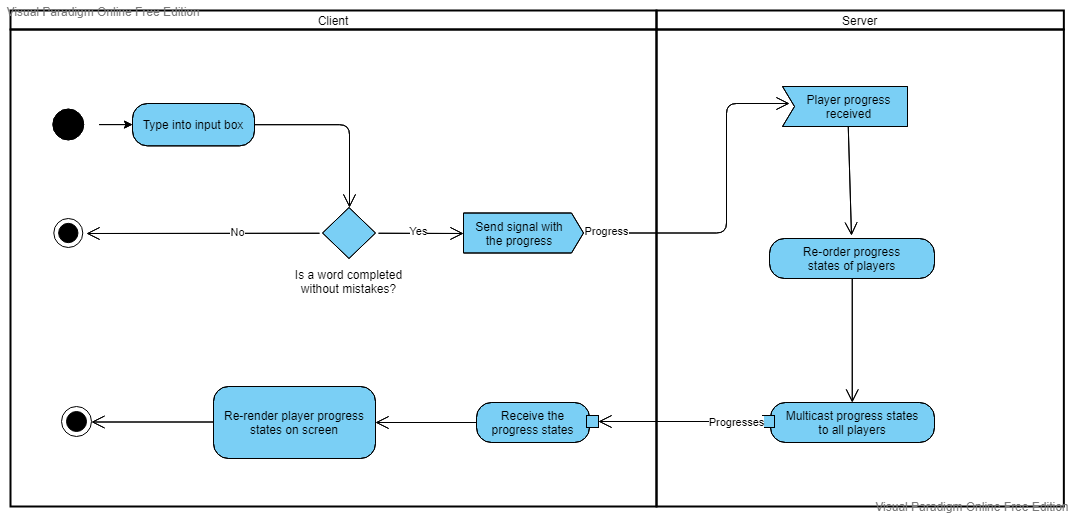
\includegraphics[width=0.79\textwidth]{activity_diagram_progress.png}
	\caption{Game progress activity diagram}
	\label{fig:progress-activity}
\end{figure}


\section{System communication}

In this section the communication between individual components is described. With help of sequence diagrams we hope to fully describe the system without leaving any place for doubts. We opted for a communication of REST and WebSockets, used whenever best suited.

REST will ensure the HTTP API is well structured and predictable. We used it in places where client-server communication is based on a single question-single answer scheme where it is not expected to be continuously asking the server for some data. Another advantage of REST is that it is ubiquitous and known by pretty much every programmer and architecture designer. Finally, many tools exist to speed up development of such REST APIs. In particular, we used one such tool to create documentation of our API.

\textbf{Swagger} tooling helped us define all schemas and endpoints of the server. The spec adheres to OpenAPI version 3 and can be found in the attachments in the \texttt{apispec.yaml} file.

However, in some parts of the program real time communication is needed and as such WebSockets were adopted in our project as the protocol used for such push-based communication. WebSocket is a web-based protocol which provides full-duplex communication over TCP, which is perfect for our real-time components such as chat, lobby, and the game. Unlike HTTP it allows two hosts to be connected in session and allows the server to push new messages without a trigger on client side. WebSockets perform client-server connection through a HTTP handshake which makes it limited to web environments. However since the creation of WebSockets many platforms have adopted them since making them a comfortable choice, even in non-web platforms.

Due to the lack of support of event based communication (which WebSocket is) in Swagger, we opted to include WebSocket schemas in the API spec anyways, but with some rules:

\begin{enumerate}
	\item WebSocket endpoints are visible as \texttt{/ws/*}
	\item WebSocket endpoints have overridden host url, because they use the \texttt{wss://} protocol instead of \texttt{https://}
	\item \texttt{GET} requests signify the initial join request
	\item \texttt{PUT} requests signify the possible client messages as a Swagger's \texttt{oneOf} object
	\item \texttt{POST} requests signify the possible server messages as a Swagger's \texttt{oneOf} object
\end{enumerate}

\subsection{Admin}

Admin panel contains many independent communication streams as it is allowed to modify various parts of the system. As seen on \figref{fig:seq-admin}, before any modifying action can be performed, the admin actor has to be authenticated. As described in the API spec we use Bearer Token based authentication where tokens are Json Web Tokens (JWTs). Each consequent admin request is required to be authorized by passing this obtained token in a HTTP header: \texttt{Authorization: Bearer <token>}. In the sequence diagram we see actions possible by the admin and the API spec describes the exact payloads.

\begin{figure}[H]
	\centering
	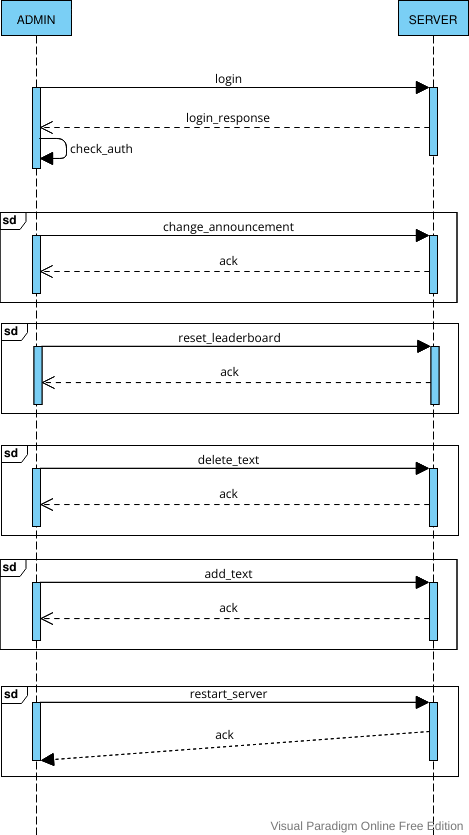
\includegraphics[width=0.63\textwidth]{seq_diagram_admin.png}
	\caption{Admin's sequence diagram}
	\label{fig:seq-admin}
\end{figure}


\subsection{Client}

\subsubsection{Lobby}

When opening the client app, user is greeted with an announcement text fetched from the server \figref{fig:seq-client-lobby}. After that user is able to set their username and join the lobby. Lobby is a place where potential players wait for other players to join to be able to start the game. In this lobby players can join and leave, which is real-time communicated to users by pushing player list updates from the server using WebSockets (indicated by a \textit{push updates} loop frame). Once the lobby countdown reaches zero, the game starts and game info is pushed to clients (such as game ID) as a final websocket message.

\begin{figure}[H]
	\centering
	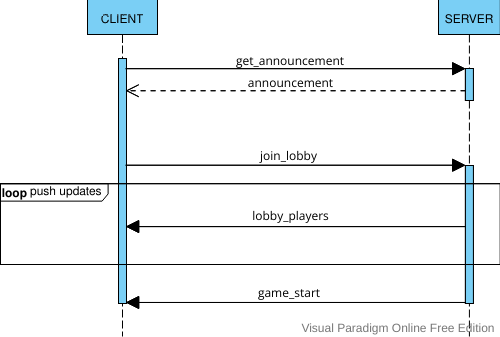
\includegraphics[width=0.8\textwidth]{seq_diagram_lobby_players.png}
	\caption{Client's lobby sequence diagram}
	\label{fig:seq-client-lobby}
\end{figure}

While in the lobby, one can choose to see the leaderboard or join the lobby chatroom to pass time.

\subsubsection{Leaderboards}

As seen in \figref{fig:seq-client-leaderboard} fetching leaderboards by a client is straightforward: the request includes a description whether the daily or all-time leaderboard is wanted, and then the appropriate leaderboard is returned as a list of usernames with their respective WPM.

\begin{figure}[H]
	\centering
	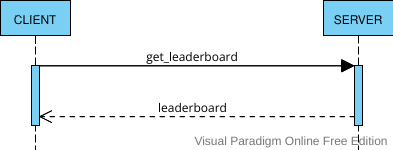
\includegraphics[width=0.8\textwidth]{seq_diagram_leaderboard.png}
	\caption{Clients's leaderboard sequence diagram}
	\label{fig:seq-client-leaderboard}
\end{figure}

\subsubsection{Chat}

The chat is simple and avoids any advanced features, after all it serves purely as a time-passer. A client actor connects to the lobby chat by establishing a WebSocket handshake with the server. Then the server is able to return new messages to all connected clients in real-time. Each message consists of user's ID and username, the message timestamp and of course the content of the message. Each client can send its own message which will be propagated to all other connected actors. Clients are free to disconnect at any time without disrupting the chat.

\begin{figure}[H]
	\centering
	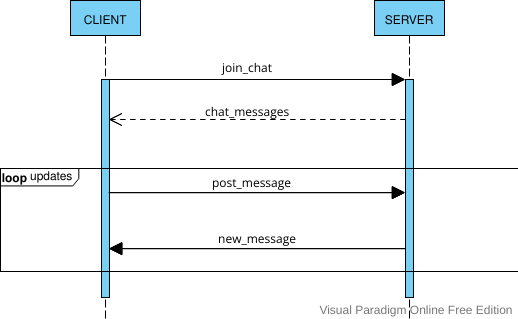
\includegraphics[width=1\textwidth]{seq_diagram_chat.png}
	\caption{Clients's chat sequence diagram}
	\label{fig:seq-chat-leaderboard}
\end{figure}

\subsubsection{Game}

Finally, there is the most important flow: the game loop. It also takes advantage of real-time capabilities of WebSockets. After the lobby each player joins the game WebSocket where each player is required to notify the game server about their progress. Progress is calculated from the character at which each player is currently at. The client update frequency is left to be implementation defined, as it plays not much of an important role (though, it is recommended to update positions after each finished word).

Game server will continuously push updated positions of all players to clients which will allow the game UI to be updated frequently. Once a player is done, they wait for all other players to finish after which all players receive the final results.

\begin{figure}[H]
	\centering
	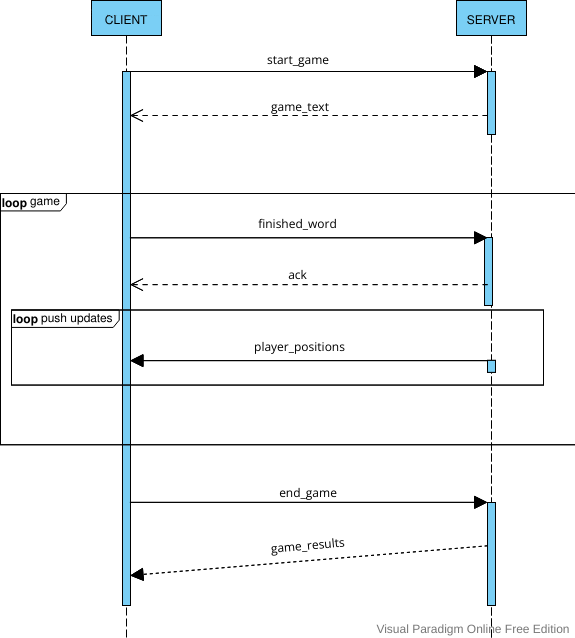
\includegraphics[width=0.8\textwidth]{seq_diagram_game.png}
	\caption{Clients's game sequence diagram}
	\label{fig:seq-game-leaderboard}
\end{figure}


\subsection{Abnormal behavior}

While using the application, some unwanted and unusual interactions can happen. Below a list of such occurrences can be found, along with an exemplary reaction from the application.

\subsubsection{Disconnected database}

An error of disconnected database could occur when trying to either read from it, or when trying to save to it. In such a case, the user should be informed about that in an error message just after a single attempt. The server never tries to connect to the database by itself, as it could make the application prone to attacks. Afterwards, the user may have another attempt.

\subsubsection{API gives no response to requests}

A user may try to communicate with the server while the API doesn't work. If there is no response from the API, the user will get an error message saying that a server connection error has occurred. On the other hand, on the server's side there would be a message for the admin with an error code, so that the server admin could figure out what the problem is.

\subsubsection{Socket can't connect}

Server will be working in the form of a loop, listening for any requests. However, a rare situation may occur when the socket can't connect, and thus the loop won't start. In that case, a connection timeout will occur and the user will be informed about the problems with the server.

\subsubsection{Insufficient resources}

In the case that there are too many requests sent to the server, we will have a situation where the given resources are insufficient. In that case, all the requests will be interrupted, and all the users trying to fetch the prediction or measurement will be informed with an error message. They will be able to try to connect again once the servers are back to normal.

\subsubsection{Malformed API request}

In some specific cases, there may be a situation when a user tries to send a malformed, unrecognizable request. In that case, a simple message with \texttt{400} code is returned.

\newpage

\section{User simulations}

To show that application works, we shall describe some steps to perform activities alongside with expected results.

\subsection{Player Simulation}
\begin{enumerate}
	\item After visiting the website the user will be asked to enter their name.
	\item After entering a name the user will be asked to select a server to connect to. Once a server is selected a connection should be established and the user should be taken to the lobby screen where an announcement, a chat box and a countdown is displayed. There should also be an option to view the leaderboards.
	\item When the user types a valid message in the chat box the message should be sent to the server and then received back since it's valid and displayed in the chat box among all other messages sent by all users.
	\item When the user types an invalid message containing a forbidden word or phrase in the chat box the message should be sent to the server and then a "<message deleted>" message should be received back since the original message was invalid, and displayed in the chat box among all other messages sent by all users.
	\item When the user chooses to see the leaderboards the leaderboard should be displayed in place of the chat box. There should be an option to switch between the daily and all-time leaderboards and both should be displayed correctly.
	\item When the countdown in the lobby reaches zero the game should start.
	\item In the game screen the following should be displayed: The text to be typed by the user, an input box where the text will be typed, the progresses of other players and the DNF (did-not-finish) countdown which displays the time left to finish typing. The other players' progresses should include the player viewing the screen, the player ranking 1st and the player ranking last, along with their WPM (words-per-minute) scores for the current game.
	\item When the user types in a word without mistakes that that word should become uneditable and marked with a different color to indicate that it was typed without mistakes. The player's progress should be sent to the server and the new progress states of all players should be received from the server, updating the progress of other players on the client screen.
	\item When the player completes typing the text without any mistakes, the game should end for them, they should be notified of their final score in WPM and their ranking among other players. The chat box should be displayed.
	\item  When the player cannot complete typing the text until the DNF timer reaches zero, the game should end, they should be notified of their final score in WPM and their ranking among other players. The chat box should be displayed.
	\item If a player scores a high score in a game, they should be notified and their name and score should be automatically entered in the leaderboard(s).
	\item When a game ends the player should be moved to the lobby. And a new countdown should be displayed to indicate when the next game begins.
\end{enumerate}

\subsection{Admin Simulation}

\begin{enumerate}
	\item After visiting the website the user will be asked to enter their login credentials. If the credentials are incorrect the user should be notified and not allowed to proceed. If the credentials are valid the user is logged in to the admin panel and the main page showing the service status as "started" or "stopped", a "Logout" button as well as the following admin options is displayed where the user can choose which action to carry out.
	\item If the user clicks on the "Service Actions" button on the main page they should be taken to the service actions page. Clicking the "Home" button should take the user to the main page and these service options should displayed:
	      \begin{itemize}
		      \item \textbf{Start Service:} If the game service is not running it should come online and users should be able to play a game when this option is clicked.
		      \item \textbf{Stop Service:} If the game service is running it should stop and users should not be able to play a game when this option is clicked.
		      \item \textbf{Restart Service:} This option should briefly stop and then restart the game service.
	      \end{itemize}
	\item If the user clicks on the "Announcement" button on the main page  they should be taken to the edit announcement page.  The currently set announcement as well as a "Home" button should be displayed. Clicking the "Home" button should take the user to the main page. Clicking the "Edit Announcement" button should display an edit box containing the current announcement. Clicking the "Save" button should set save the contents of the edit box as the new announcement and any user logging in to the game and viewing the lobby screen should be able to see this new announcement. Clicking the "Cancel" button should remove the edit box and only display the announcement.
	\item If the user clicks on the "Leaderboard" button on the main page they should be taken to the leaderboard page. The current leaderboards as well as a "Home" button should be displayed. Clicking the "Home" button should take the user to the main page. Clicking the "Reset" button should display a confirmation box with "Confirm" and "cancel" options. Clicking the "Confirm" button should clear the all-time leaderboard data and go back to displaying the empty leaderboards.  Any user logging in to the game and viewing the leaderboard should be able to see that the leaderboard has been cleared. Clicking the "Cancel" button should remove the confirmation box.
	\item If the user clicks on the "Content Manager" button on the main page they should be taken to the content management page which will display two options: "Browse content" and "Add content". Also a "Home" button should be displayed, which, when clicked, should take the user to the main page.
	\item If the user clicks on the "Browse Content" button on the content manager page they should be taken to the browse content page, where the content entries in the database, ordered by the date of their addition to the database, as well as "Back" and  "Home" buttons should be displayed. Clicking on the "Back " button should take the user back to the content manager page and clicking on the "Home" button should take the user back to the main page. Two input fields "search by ID" and "search by phrase" should be available and the user should be able to search the database content based on the Id number of a content entry or a search phrase they enter. When the "Search" button is clicked the content entries matching the search criteria should be displayed, with a "Delete"  button next to each entry. Clicking the "Delete" button should display a confirmation box with "Confirm" and "cancel" options. Clicking the "Confirm" button should delete the entry from database and any user logging in to the game should not be given the deleted entry as a text afterwards.
	\item If the user clicks on the "Add Content" button on the content manager page they should be taken to the add content page, where the add content options, as well as "Back" and  "Home" buttons should be displayed. Clicking on the "Back" button should take the user back to the content manager page and clicking on the "Home" button should take the user back to the main page. Two buttons "Add From Text" and "Add From File" should be available and the user should be able to to add new content to the database using these buttons. After entering a text or choosing a .txt file to be processed and clicking "save" the newly added content should be displayed at the top of the list of entries shown on the content manager page and user logging in to the game should have a chance to be given the newly added entry as a text afterwards. In the case that the .txt file selected is invalid the user should be notified that there are errors in the file it cannot be read.
	\item When the user clicks on the "logout" they should be taken to the login page where the input box for the login password has been cleared. Clicking on "login" without entering password should not log the user back in.
\end{enumerate}

\section{Technology proposal}

First of all we would like to stress that the technology used will not matter. When designing the project we made sure to be as technology and platform agnostic as possible. That being said, we have some preference which will be presented in the following paragraph. However these are merely suggestions, and should not be strictly adhered to.

We believe creating a web app for the admin panel makes most sense. Admin panel does not have to be quickly accessible (for example from mobile) as it contains no time sensitive settings. Responsive design will not be needed either since it is primarily for desktop devices. However if one was to add responsive design, turning this admin panel to a PWA could be a nice addition. As to technology, any modern light client framework/library will do just fine (such as Vue/Preact/Svelte), Angular is not recommended due to its large size. It would be important however to use TypeScript instead of JavaScript since it provides static typing and therefore is less prone to runtime errors. Finally, the web app could be powered by some meta framework which would provide server-side-rendering (Nuxt/Next).

Nowadays pretty much any language can be used for backend development. However, lately there has been a boom of new systems languages appearing and completely redefining the scene. One such language which would be of our recommendation is Rust. It provides safety of a high level languages while maintaining speeds on par with C. It does not carry a heavy runtime (like Java, C\#, or Python) making it easy to deploy on low end devices. One important factor that has to be considered is WebSocket support, luckily Rust does have packages implementing the WebSocket protocol so it will not cause any problems. For a database we recommend using relational databases. Some free  solution, such as PostgreSQL or MySQL will be perfect for the job.

Finally for the client app instead of recommending a stack, we would like to recommend against one: web. Purpose of this project was to be platform independent, ideally many clients would be created each on a completely different platform while still being able to coexist and play games together. Web is not recommended since it is the obvious (and boring) choice. Get creative! Examples include terminal apps, native desktop apps, discord bot, etc.

\section{Attachments}

\begin{enumerate}
	\item \textattachfile[color=0 0 1]{apispec.yaml}{apispec.yaml} -- OpenAPI v3 specification of the API
\end{enumerate}


\end{document}
